% 5) Methods - provide a description of the way in which you intend to address the research question.  This means describing the existing tools/systems that you will use, new tools or systems that you will build and the experiments that you will conduct.
\section{Results}
\subsection{Harpocrates}
We designed a system, Harpocrates (Greek god of silence, secrets, and confidentidality), which allows users to easily compensate publishers at a fair rate for their content.
Harpocrates is composed of a client-side browser extension for users and a server for accounting.
Furthermore, it fits into the current ad ecosystem with minimal implementation work required for publishers.

\subsubsection{Design Considerations}
In designing Harpocrates, there was a clear set of requirements whic, if not accomplished, would yield a system infeasible for wide deployment.
First, it must address the needs of current ad-blocker users, else they would not consider using it.

It must also be unobtrusive and get our of the user's way.
For example, with our current design, there is a very simple settings page that allows the user to pick a budget, etc.
The rest of the logic happens erver-side, improving user experience.

Performance must improve over the current Web experience without an ad-blocker.
Surveys show that a substantial proportion of users use ad-blockers for performance reasons~\cite{hubspot2016adblock}, so any substitute should strive to address that concern specifically.

The system should fit into the current Web ecosystem, i.e. must not rely on any new standards in order for it to see wide adoption.
Correspondingly, the implementation cost for publishers must be minimized, because it will never see wide adoption without publishers' acceptance.
This means that solutions that involve adding server-side code, such as would be required to enable many of the services described in Section ~\ref{academic_related}.

Finally, it must provide control over the browsing experience for both users and publishers alike.
Currently, publishers are essentially locked in to using a combination of subscription and ad tactics for revenue.
By enabling them to recoup some of the lost revenue due to blockers, and enabling users to opt-in to funding their favorite content, both parties benefit.

\subsubsection{Architecture}
Our solution relies on fact that ad exchanges are efficient marketplaces for determining the fair value for a given piece of real estate on the internet.
In order to take advantage of this fact, Harpocrates sits inline in the ``waterfall'' (Figure ~\ref{fig:waterfall}).

\begin{figure}[h]
\centering
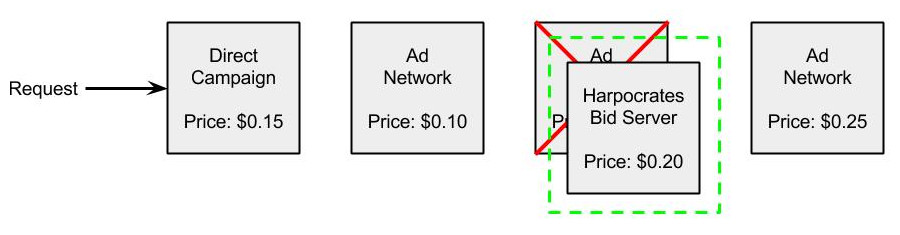
\includegraphics[width=0.5\textwidth]{waterfall}
\caption{Harpocrates sits inline with the current ad exchange ecosystem.}
\label{fig:waterfall}
\end{figure}

From the publisher's point of view, Harpocrates is essentially another ad network, which, given an impression, returns a bid for the ad (or none).
Hence, its implementation cost is no higher than that of adding another ad network for a given publisher.

From the user's point of view, Harpocrates is simply a browser extension.
Given a number of initial settings (Figure ~\ref{fig:harpocrates_ui}), Harpocrates will make bids on the user's behalf for a given ad.

\begin{figure}[h]
\centering
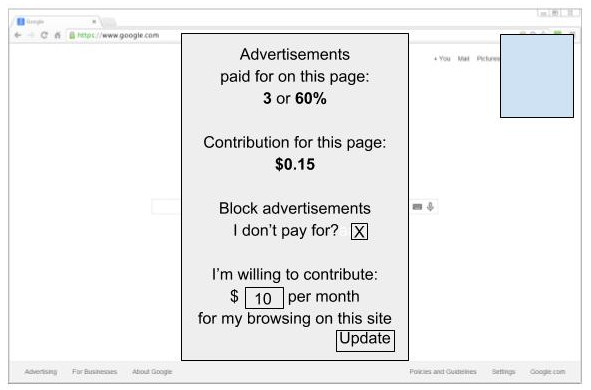
\includegraphics[width=0.5\textwidth]{harpocrates_ui}
\caption{For the user, Harpocrates simply requires installing a browser extension and initializing a few settings.}
\label{fig:harpocrates_ui}
\end{figure}

Finally, Harpocrates also acts as a clearinghouse, settling account monthly.
for a given set of publishers $N$ and users $M$, only $O(|N| + |M|)$ payments need to be transacted (i.e. one payment from each user to Harpocrates, and one payment from Harpocrates to each publisher).
At scale, we gain a lot from doing these macropayments: in the worst case, these users and publishers would result in $O(|N| \cdot |M|)$ payments (one for each user/publisher pair).

These aspects of the architecture make Harpocrates a good candidate solution, given the aforementioned design considerations.
It addresses the needs of current ad-blocker users by showing them fewer ads.
The user interface makes it practically invisible from a user's point of view.
Performance is improved by eliminating a whole round-trip to the ad CDN (Figure ~\ref{fig:harpocrates}).
It fits into the ecosystem, requiring no new standards.
Finally, the implementation is simply adding another ad network, minimizing implementation costs.

\begin{figure}[h]
\centering
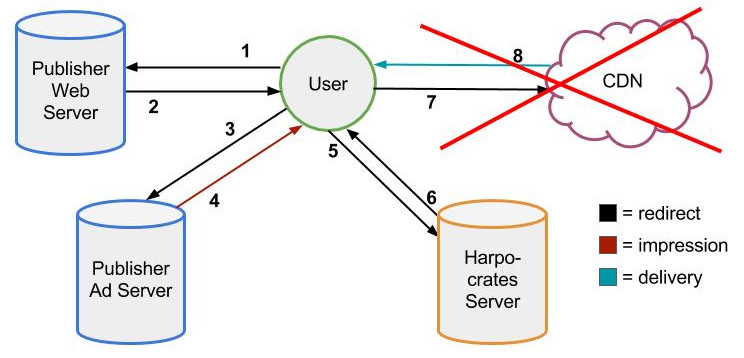
\includegraphics[width=0.5\textwidth]{harpocrates}
\caption{Harpocrates cuts out a whole roundtrip request to the ad server CDN, improving performance.}
\label{fig:harpocrates}
\end{figure}

\subsection{\textit{Un}acceptable Ads}
\textit{Un}acceptable Ads is a proof of concept to illustrate anothr path forwards for users who block ads because of the reduced performance and/or visual obtrusivness.
We have modified two Chrome extensions to include a ``tolerance'' specified by the user, which corresponds to the percent of ads they are willing to see (we note that this does \textit{not} address the needs of users whose foremost concern is privacy, and leave that for future work).

\subsubsection{uBlock Origin}
uBlock Origin is a popular ad-blocker with nearly 9 million installs on Google Chrome as of May 2017.
It works by blocking network requests which match against a list of known advertising URL's (e.g. EasyList~\cite{easylist}).
We modified the extension to allow the user to specify their tolerance for ads, resulting in probabilistic blocking of ad requests.

\subsubsection{Perceptual Blocker}
Storey, et al.~\cite{storey2016future} recently published work on what they dubbed a ``perceptual blocker'', which blocks ads based on their content rather than simply the structure of the page.
We modified this extension similarly to take a tolerance level and a few other parameters (Figure ~\ref{fig:unacceptable_ui}), and probabilistically overlay a green box where ads would otherwise be shown (Figure ~\ref{fig:unacceptable}).

\begin{figure}[h]
\centering
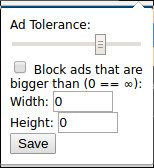
\includegraphics[width=0.15\textwidth]{unacceptable_ui}
\caption{User interface for our modification of the Perceptual Blocker.}
\label{fig:unacceptable_ui}
\end{figure}

\begin{figure}[h]
\hfill
\subfigure{
\includegraphics[width=0.15\textwidth]{unacceptable_no_tolerance}}
\hfill
\subfigure{
\includegraphics[width=0.15\textwidth]{unacceptable_high_tolerance}}
\hfill
\caption{\textit{Un}acceptable Ads allows the user to select their tolerance for advertisements, from 0\% (left) upwards (right).}
\label{fig:unacceptable}
\end{figure}

\subsubsection{Summary and Technical Challenges}
These extensions serve as proofs of concept for a new generation of ad-blockers which allow for a more fine-grained tuning of what types of ads should be blocked.
This approach can provide partial or full compensation for the publisher while preventing the user from the performance and/or visual issues associated with ads.

\subsection{Performance}
In order to assess the impact of ad-blockers on performance, we performed an experiment to measure page load times across five popular sites, with and without uBlock Origin enabled.
For each page, we took the average of five measurements of page load time (gathered from the Chrome extension Page Load Time~\cite{pageloadtime}).
The results backed up survey findings that many users use ad-blockers for performance reasons~\cite{hubspot2016adblock}, as there was a 2.33x speedup with uBlock enabled (Figure ~\ref{fig:load_times}).

\begin{figure}[h]
\centering
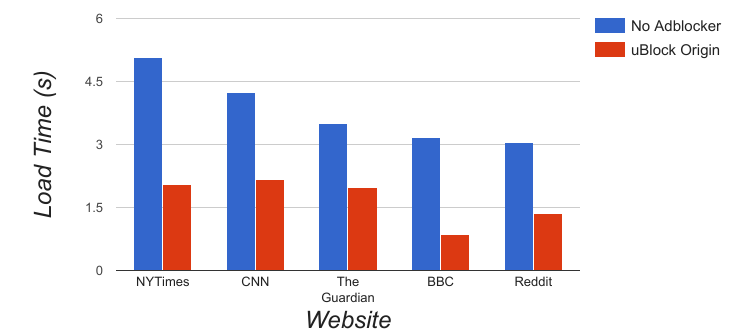
\includegraphics[width=0.5\textwidth]{load_times}
\caption{Loading times for five popular websites with and without the popular ad-blocker uBlock Origin.}
\label{fig:load_times}
\end{figure}

To assess the performance of our \textit{Un}acceptable Ads extensions, we performed a similar experiment by measuring page load times for the Chicago Tribune homepage at multiple different levels of ad tolerance.
Our findings are consistent with our intuition: since uBlock blocks based on network requests, performance should decrease as tolerance goes up.
For the Perceptual Blocker, however, performance stays relatively constant regardless of tolerance, since ads are detected and hidden after they are loaded (Figure ~\ref{fig:load_times_over_range}).

\begin{figure}[h]
\centering
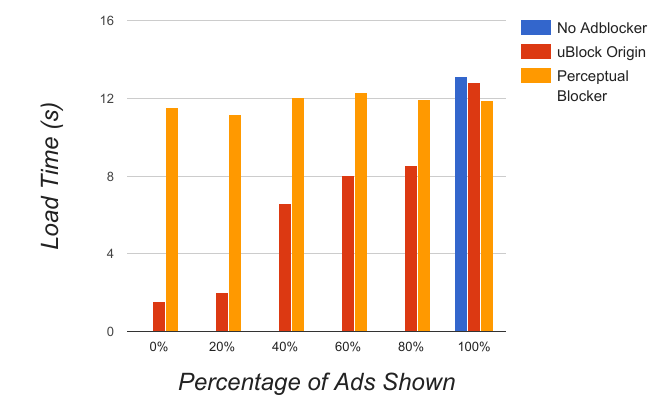
\includegraphics[width=0.5\textwidth]{load_times_over_range}
\caption{Loading times for Chicago Tribune homepage with varying levels of tolerance for ads using the \textit{Un}acceptable Ads extension (``Perceptual Blocker'') and a modified version of uBlock Origin.}
\label{fig:load_times_over_range}
\end{figure}